\PassOptionsToPackage{quiet}{fontspec} % 抑制中文字体警告
\documentclass[12pt,AutoFakeSlant,AutoFakeBold]{article}
\usepackage{ctex}
\usepackage[a4paper,top=2.5cm,bottom=2.5cm,left=2.5cm,right=2.5cm]{geometry}

% Useful packages
\usepackage{amsmath}
\usepackage{graphicx}
\usepackage[colorlinks=true, allcolors=blue]{hyperref}
\usepackage{booktabs}
\usepackage{subfigure}
\usepackage{enumitem}
\usepackage{minted}
\usepackage{multirow}
\usepackage{titlesec}
\usepackage{amsfonts}
\usepackage{longtable}
\usepackage{gbt7714}
\usepackage{mdwlist}
\titleformat*{\section}{\Large\itshape\centering}
\newtheorem{theorem}{定理}
\newtheorem{lemma}{引理}

\newcommand{\nor}{\oplus}

\begin{document}

\centerline{\Large\heiti\textbf{关于特定棋子颜色问题的讨论}}

\vspace{0.3cm}

\centerline{\large\heiti\textbf{摘要}}

这篇文章研究一种,通过指定的规则,进行状态转移的黑白棋游戏。

我们首先通过将$n$个子的黑白棋序列抽象为$n$为的二进制数,然后通过异或运算和循环位移操作,描述了其状态转移的方式。

然后我们通过数学建模分析,重点分析其进入特殊状态(全黑和进入循环)的情况,并得到以下结论:

\begin{enumerate*}
    \item 如果,棋子的个数为$2^n$,其中$n$为自然数,则在进行$2^n$次操作后,会进入全是黑棋的状态;
    \item 如果,棋子的个数为$m$个,其中$m$为奇数,则如果能找到一个自然数$N$,使得$N$满足$N=2^n=km+1$,其中,$n$和$k$为任意自然数。则这个系统执行$N$次后的状态,必然与执行$1$次后的状态相同,也就是会陷入循环。同时,我们利用欧拉定理,我们论证了这样的$N$必然存在;
    \item 如果棋子的个数为$2m$,其中$m$为正整数,且$m$个子的系统拥有对所有开始情况都适用的循环周期,且第一次循环开始于第$i$次执行,第二次循环开始于第$j$次执行。则这个系统也拥有对所有的开始情况都适用的循环周期,且第一次循环开始于第$2i$次执行,第二次循环开始于第$j$次执行。
\end{enumerate*}

这样,我们完成了对任意棋子数量的黑白棋系统的讨论。

最后,我们讨论了模型的推广,我们认为我们的建模方法可以推广到其他的适合用二进制数表示状态的情况。

\textbf{关键词:} 异或、循环位移、状态转移

%%%%%%%%%%%%%%%%%%%%%%%%%%%%%%%%%%%%%%%%%%%%%%%%%%%%%%%%%%%%%%%%%%%%%%%%%%%%%%%
%                                                                             %
%%%%%%%%%%%%%%%%%%%%%%%%%%%%%%%%%%%%%%%%%%%%%%%%%%%%%%%%%%%%%%%%%%%%%%%%%%%%%%%

\newpage

\section{问题重述}

考虑一个由$N$个黑色和白色棋子组成的圆形排列。根据以下规则进行操作:如果相邻的两个棋子颜色相同,则在它们之间放置一个黑色棋子;如果相邻的两个棋子颜色不同,则放置一个白色棋子。完成一圈中所有可能的放置后,移除原始圈中的所有棋子。然后,重复上述过程,新一圈的棋子基于上一次形成的圈中棋子的颜色排列。本文旨在探讨,经过多次这样的重复操作后,棋子的颜色分布将如何变化。

\section{符号说明}

\begin{table}[h]
    \centering
    \caption{符号说明}
    \begin{tabular}{ccc}
        \toprule
        符号 & 符号说明 & 备注 \\ 
        \midrule
        $\nor$ & 异或 & ~ \\
        $R(X,n)$ & 循环右移 & 将二进制数$X$循环右移$n$位\\
        $a_0$ & 棋子的初始状态 & ~ \\ 
        $a_n$ & $R(a_0,n)$ & 将$a_0$循环右移$n$位
        \\ \bottomrule
    \end{tabular}
\end{table}

\section{数学模型的建立}

我们可以用一个二进制数来表示当前的棋子颜色,我们用$1$表示白色,$0$表示黑色,例如“黑、白、黑”,可以用二进制数$010$表示。那么,我们可以发现,不同表示白色,相同表示黑色,这正好符合异或运算的定义。

对于一个有$n$个棋子的情况,我们可以用一个$n$位的二进制数去表示这些棋子在某一时刻的状态。假设,$t$时刻,棋子的状态可以用二进制数$b_t$表示,那么在$t+1$时刻的状态可以如下表示:
\begin{equation}
    b_{t+1} = b_{t}\nor R(b_{t},1)
\end{equation}
其中,$R(b_{t},1)$表示,将$b_{r}$循环右移一位。

循环右移是计算机科学中一种常见的操作,它涉将数据结构中的元素向右移动指定的位置数,而最右侧的元素则循环移动到最左侧。

如上面那个例子,对于一个“黑、白、黑”的棋子分布,在按照题目要求进行一次操作后,会变为“黑、白、白”。而其对应的二进制数为$010$,将其循环右移一位的结果是$001$,两者进行异或可以得到$011$,也就是“黑、白、白”所对应的二进制数。

\section{数学模型的求解}

\subsection{异或运算的性质}

异或运算的以下性质,接下来我们会用到:

\begin{itemize*}
    \item 交换律:
    \begin{equation}
        A\nor B=B\nor A
    \end{equation}
    \item 结合律:;
    \begin{equation}
        A\nor (B \nor C) = (A\nor B) \nor C
    \end{equation}
    \item 恒等律:
    \begin{equation}
        A\nor 0=0\nor A=A
    \end{equation}
    \item 归零律:
    \begin{equation}
        A\nor A=0
    \end{equation}
\end{itemize*}

\subsection{循环右移操作的性质}

根据循环右移操作的定义,我们可以轻松地得到下面几条性质,我们在这里不进行证明:

\begin{itemize*}
    \item 将一个数先循环右移$m$位,再循环右移$n$位,等价于直接将其循环右移$m+n$位:
    \begin{equation}
        R(R(A,n),m) = R(A,n+m)
    \end{equation}
    \item 将一个$n$位的二进制数,循环右移$n$位是其自身。假设$A$是一个$n$位的二进制数:
    \begin{equation}
        A = R(A,n)
    \end{equation}
    \item 从上一条可以推论,假设$A$是一个$n$位的二进制数,$k$是一个整数:
    \begin{equation}
        R(A,m)=R(A,m+kn)
    \end{equation}
    \item 由于异或运算是按位操作,所以在异或前循环右移还是在异或后循环右移没有区别,也就是:
    \begin{equation}
        R(A\nor B,m) = R(A,m)\nor R(B,m)
    \end{equation}
\end{itemize*}

\subsection{引理}

\begin{lemma}
    设开始时,黑白子对应的二进制数为$a_0$,$a_n$表示$R(a_0,n)$。假设其现在的状态为$a_0\nor a_{2^m}$,则经过$2^m$次操作后,其状态会变为$a_0\nor a_{2^{m+1}}$。
\end{lemma}

证明如下:设$G$为二进制数的集合,由于$\nor$满足结合律,则代数系统$<G,\nor>$是一个半群,可以在上面定义乘幂运算。
\begin{itemize*}
    \item 进行一次操作之后,状态变为$a_0\nor a_1 \nor a_{2^m} \nor a_{2^m+1}$;
    \item 进行两次操作之后,状态变为$a_0\nor a_1^2 \nor a_2 \nor a_{2^m} \nor a_{2^m+1}^2 \nor a_{2^m+2}$;
\end{itemize*}

我们注意由$a_0$所产生的所有项,进行一次操作后,其产生了一个$a_1$,本身不变,再进行一次操作后,$a_1$本身留下,$a_2$由$a_1$产生,这种次数的传递方式,与杨辉三角形所一致,如图\ref{fig:杨辉三角}所示。

\begin{figure}[!ht]
    \centering
    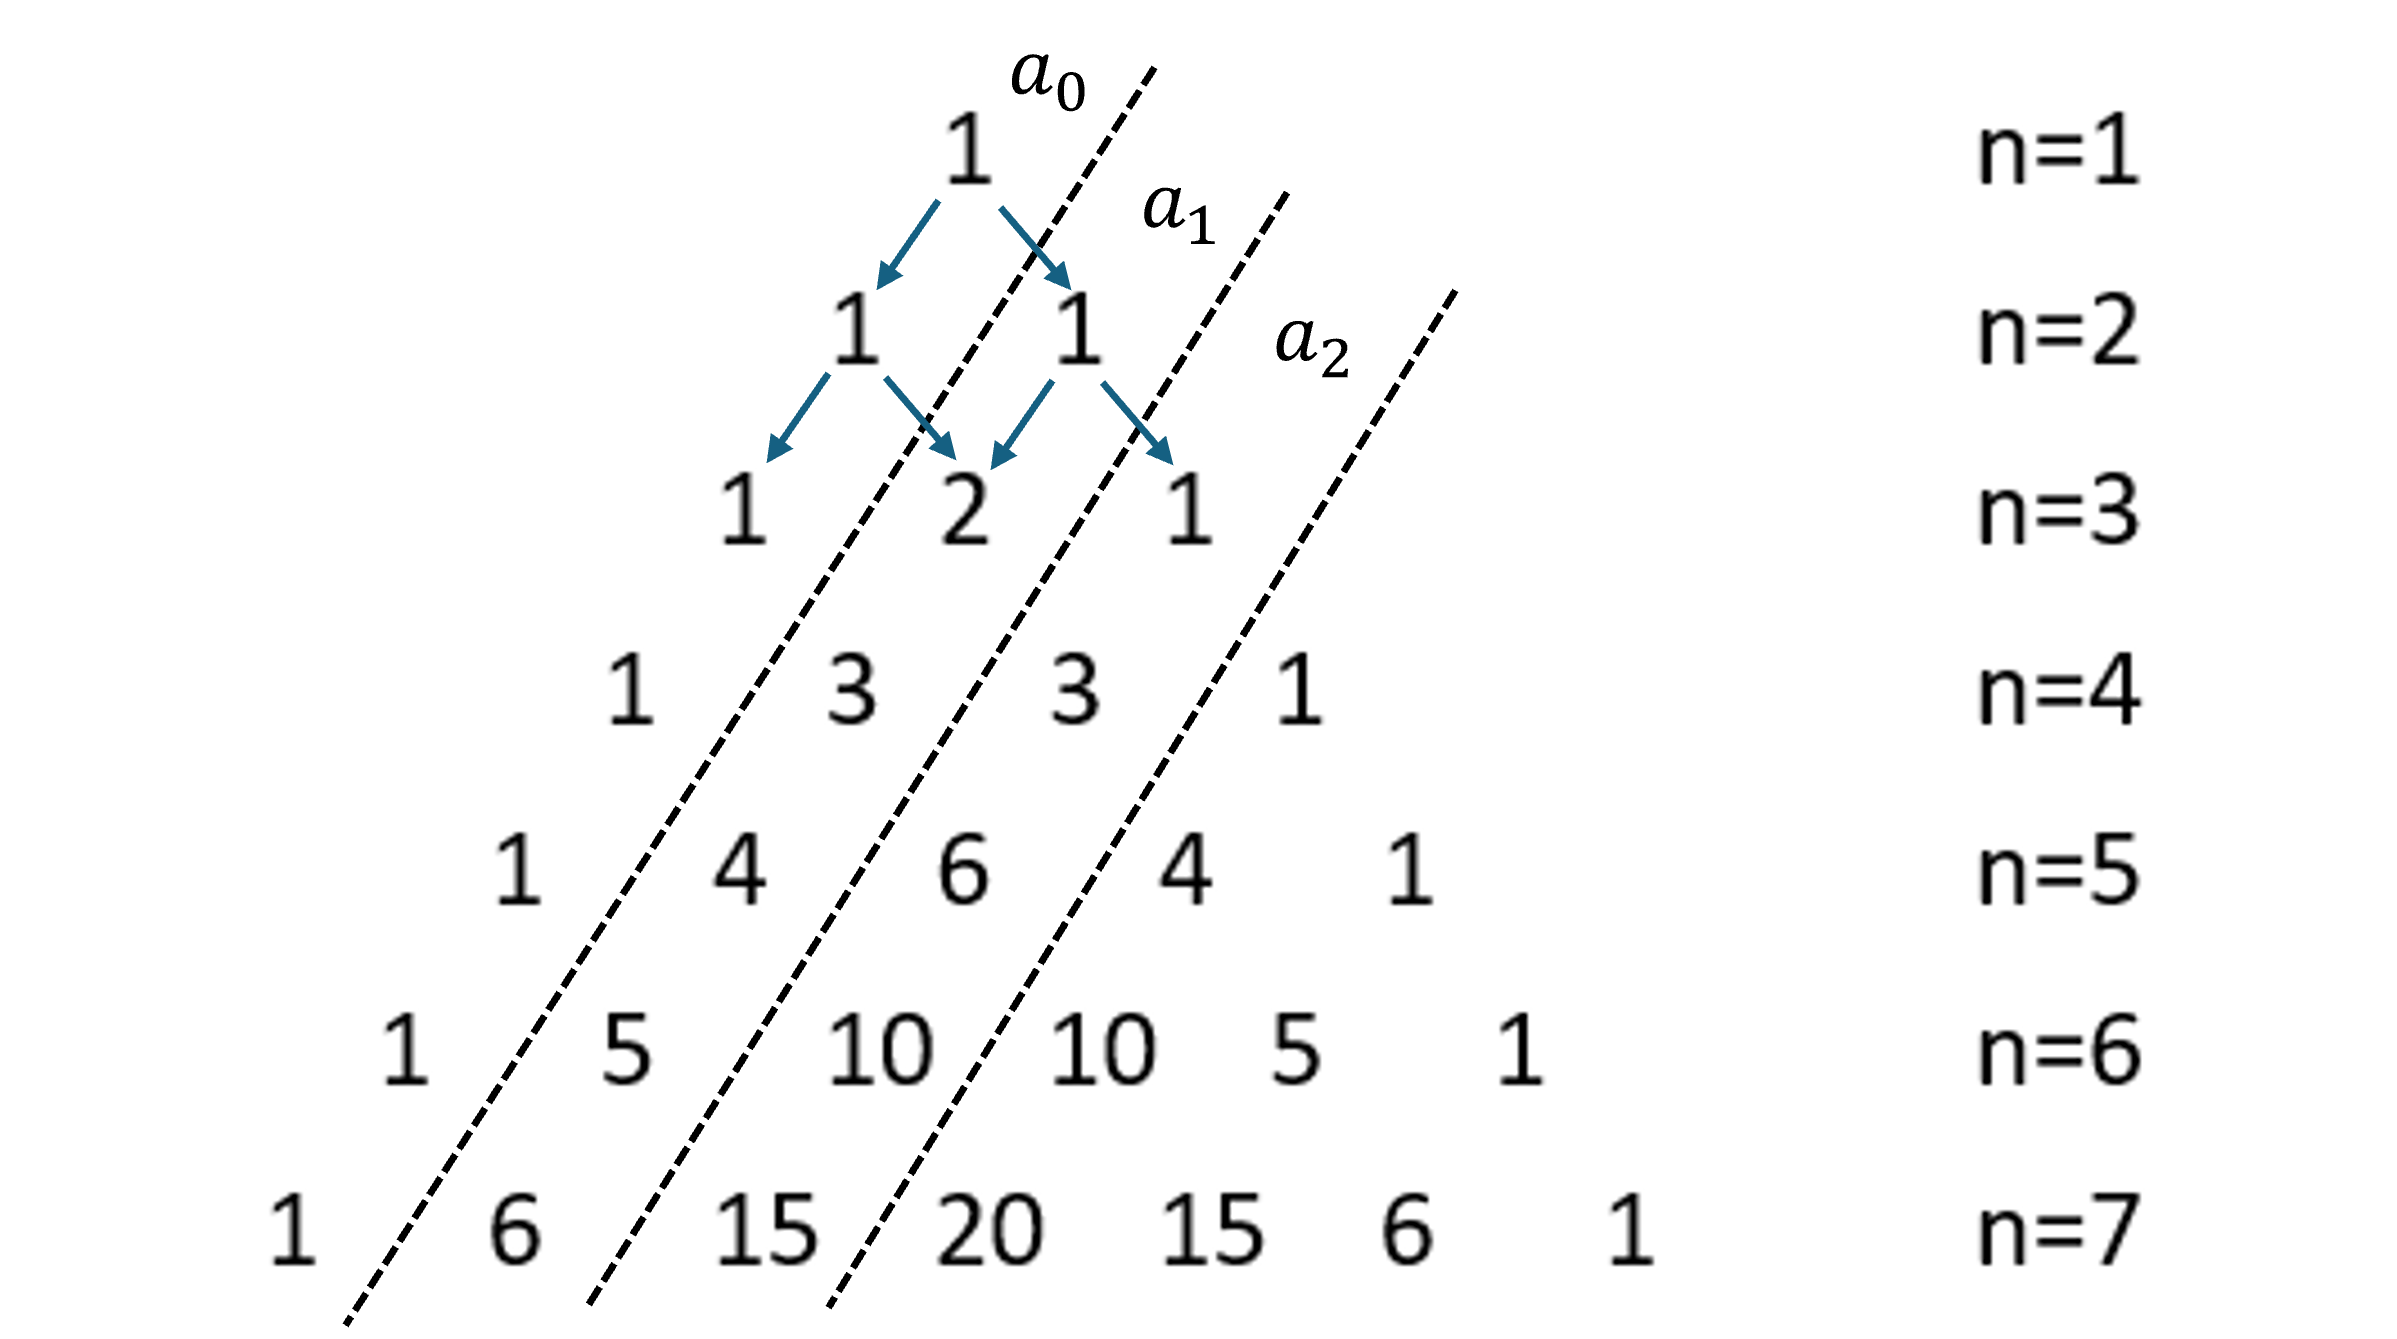
\includegraphics[width=0.8\textwidth]{图片1.png}
    \caption{次数传递方式}
    \label{fig:杨辉三角}
\end{figure}

所以由$a_0$所产生的所有项,在$2^m$次操作后,对应的次数为杨辉三角形的第$2^m+1$行。杨辉三角形的$2^m$行均为奇数\cite{hinz1992pascal},则除首尾外,第$2^m+1$行的元素均为2个奇数的和,应当为偶数。

根据$\nor$运算的归零率,偶数项均为0,则$a_0$在$2^m$次操作后,得到$a_0\nor a_{2^m}$,同理,$a_{2^m}$在进行$2^m$次操作后,得到$a_{2^m}\nor a_{2^{m+1}}$。所以,$a_0\nor a_{2^m}$,经过$2^m$次操作后,其状态会变为$a_0\nor a_{2^m}^2 \nor a_{2^{m+1}}$,而$a_{2^m}^2=0$。所以,$a_0\nor a_{2^m}$,经过$2^m$次操作后,其状态会变为$a_0\nor a_{2^{m+1}}$。

\subsection{循环周期}

\begin{theorem}
对于一个$m$个子的黑白棋系统,无论其初始状态为何,如果能找到一个数$N$,使得$N$满足$N=2^n=km+1$,其中,$n$和$k$为任意自然数。则对于这个系统,从初始状态开始,进行$N$次操作后的状态,必然与进行一次操作后的状态相同。
\end{theorem}

证明如下:对于任意黑白棋系统,进行一次操作后的状态必然是$a_0\nor a_1$,根据引理,再执行一次操作(也就是共执行两次操作后),状态变为$a_0\nor a_2$,再根据引理,再执行两次操作(也就是共执行四次操作后),状态变为$a_0\nor a_4$。以后类推,执行$N$次操作后,状态变为$a_0\nor a_N$。又因为有
\begin{equation}
    R(A,m)=R(A,m+kn)
\end{equation}
且
\begin{equation}
    N=km+1
\end{equation}
所以
\begin{equation}
    a_1=a_N
\end{equation}
所以,如果存在这样的数$N$,则对于任意一个起始状态,执行$N$次操作后,必定得到和执行1次操作后相同的状态,并开始循环。根据起始状态的不同,和$m$的大小,循环可能提前开始,但是一但到达$N$次,循环必然开始。

我们很容易注意到,对于偶数个棋子的系统,这样的$N$是不可能存在的,但是我们依然有办法去寻找其循环周期,这将在之后进行讨论。

我们现在讨论对于奇数个棋子的系统,这样的$N$是否必然存在。假设对于一个$m$个棋子的系统,$m$是一个奇数,则其一定与2互质,也就是$\gcd(2,m)=1$,那么我们利用欧拉定理可以得到:

\begin{equation}
    2^{\varphi(m)}\equiv 1(\mod m)
\end{equation}
其中,$\varphi(m)$表示,小于$m$且与$m$互质的自然数的个数,其一定是一个自然数。所以我们取

\begin{equation}
    N = 2^{\varphi(m)}
\end{equation}
则$N$一定是满足条件的(但可能不是最小的),所以满足条件的$N$必然存在。

\begin{theorem}
    如果一个$m$个子的黑白棋系统对任意起始情况都适用的循环周期,且第一个循环开始于第$i$步操作,第二个循环开始于第$j$步操作。则一个$2m$个子的黑白棋系统也有对任意起始情况都适用的循环周期,且第一个循环开始于第$2i$步操作,第二个循环开始于第$2j$步操作。
\end{theorem}

证明非常简单,对于任意一个状态$A$,执行一次操作之后,状态为$A\nor R(A,1)$,执行两次操作后,状态变为$A\nor R(A,2)$,这相当于,将这个$2m$个子的黑白棋系统,按照奇偶分为两个$m$个子的系统,并进行一次操作。也就是说,对于这个$2m$个子的黑白棋系统而言,执行两次操作,相当于对两个$m$个子的黑白棋子系统执行一次操作。那么当两个子系统都进入循环后,这个$2m$个子的黑白棋系统也会进入循环。

\subsection{\texorpdfstring{$2^n$}{2\^n}个子的情况}

从上面的讨论中我们可以发现,对于$2^n$个子的黑白棋系统不在我们的讨论范围内。我们对其进行单独讨论。

对于2个子的情况,我们从任意情况$a_0$开始:

\begin{itemize}
    \item 执行一次操作后:$a_0\nor a_1$
    \item 执行两次操作后:$a_0\nor a_1^2 \nor a_2 = a_0^2 \nor a_1^2 = 0$
\end{itemize}

也就是说,对于2个子的情况,执行2次操作后,必然进入全黑的情况。

对于4个子的情况,我们可以仿照定理2的证明方法,其执行2次等价于其按照奇偶分开的两个2个子的系统分别执行1次。那么$2\times 2 = 4$次执行后,也会进入全黑情况。

使用数学归纳法不难得出,对于$2^n$个子的情况,执行$2^n$步后,必然进入全黑的情况。

\subsection{总结}

我们对于一个任意数量个棋子,采取任意初始状态的黑白棋系统进行的讨论,讨论了其是否进入全黑状态,如果不进入全黑状态,则是否会进入循环情况的分析,其总结如下:

\begin{enumerate*}
    \item 如果,棋子的个数为$2^n$,其中$n$为自然数,则在进行$2^n$次操作后,会进入全是黑棋的状态;
    \item 如果,棋子的个数为$m$个,其中$m$为奇数,则一定能找到一个自然数$N$,使得$N$满足$N=2^n=km+1$,其中,$n$和$k$为任意自然数。这个系统执行$N$次后的状态,必然与执行$1$次后的状态相同,也就是会陷入循环。
    \item 如果棋子的个数为$2m$,其中$m$为正整数,且$m$个子的系统拥有对所有开始情况都适用的循环周期,且第一次循环开始于第$i$次执行,第二次循环开始于第$j$次执行。则这个系统也拥有对所有的开始情况都适用的循环周期,且第一次循环开始于第$2i$次执行,第二次循环开始于第$j$次执行。
\end{enumerate*}

我们注意到,上面的讨论,覆盖了所有大于等于2的自然数,也就是说,其可以处理所有的情况。

\section{计算机辅助验证}

我们编写了程序,来模拟不同棋子的情况,具体的程序见附录,表\ref{tab:模拟结果}是运行结果。

\begin{table}[!ht]
    \centering
    \caption{计算机模拟结果}
    \begin{tabular}{cccc}
        \toprule
        棋子个数 & 达到全黑步数 & 第一个循环节起始 & 第二个循环节起始 \\ 
        \midrule
        2 & 2 & —— & —— \\ 
        3 & —— & 1 & 4 \\ 
        4 & 4 & —— & —— \\ 
        5 & —— & 1 & 16 \\ 
        6 & —— & 2 & 8 \\ 
        7 & —— & 1 & 8 \\ 
        8 & 8 & —— & —— \\ 
        9 & —— & 1 & 64 \\ 
        10 & —— & 2 & 32 \\ 
        11 & —— & —— & —— \\ 
        12 & —— & 4 & 16 \\ 
        13 & —— & —— & —— \\ 
        14 & —— & 2 & 16 \\ 
        15 & —— & 1 & 16 \\ 
        16 & 16 & —— & —— \\ 
        \bottomrule
    \end{tabular}
    \label{tab:模拟结果}
\end{table}

其中,11个棋子和13个棋子的情况,达到128次迭代上限时,没有找到循环。我们可以看到,对于$2^n$个棋子的特殊情况,我们的模型均准确预言了其到达全黑的步数。对于表中所有奇数个棋子的情况,所有找到循环节的,均如我们的模型所预言的,第一个循环从第1步开始,第二个循环从符合条件的第$N$步开始。对于$2m$且不是2的整数次幂的情况,也均如模型所预言的,第一个和第二个循环开始处为$m$个子的情况的对应循环开始处的2倍(观察3,6,12个子的情况,特别明显)。

\section{模型评价}

\subsection{模型优点}

我们对于黑白棋按照规则状态转换的问题的特殊情况进行了讨论,也就是进入全黑情况和陷入循环进行了重点研究。我们给出了在拥有$2^n$个棋子的情况下,棋子进入全黑状态的步数。以及在其他情况下,开始循环的步数,并给出了第一个和第二个循环开始的步数。这些讨论均是不考虑初始状态的,也就是其是对于所有的初始状态都适用的,具有非常好的普遍性。

\subsection{模型缺点}

我们的模型没有考虑初始状态的影响,很明显,特殊的初始状态会提前循环的到来,并缩短循环长度(如全黑的状态)。也没有考虑一些更加特殊的情况。

\section{模型改进与推广}

\subsection{模型改进}

我们的模型下一步的改进方向是,将特殊的初始状态纳入讨论范围,特殊的初始状态,可能会显著影响状态的转移。

\subsection{模型的推广}

我们这种将黑白子序列抽象为二进制数,然后适用异或等方式处理的思路可以推广到其他处理的对象只有两种状态的情况。异或运算的良好性质,可以极大地简便我们的运算于分析。


\newpage

\bibliographystyle{gbt7714-numerical}
\bibliography{bibtex}

\newpage
\appendix
\centerline{\Large\heiti\textbf{附录}}

\section{所用代码}

\subsection{clear\_symvar.m}

\begin{minted}{matlab}
function new_P = clear_symvar(P)
    new_P = sym(1);
    
    vars = symvar(P);
    for var=vars
        power = feval(symengine, 'degree', P, var);
        if mod(power, 2) == 0 && power > 0
            power = 0;
        end
        if mod(power, 2) == 1 && power > 0
            power = 1;
        end
        new_P = new_P .* var .^ power;
    end

end
\end{minted}

\subsection{main.m}

\begin{minted}{matlab}
clearvars

n_chess = 127;
n_iteration = 256;

% 初始化最开始的状态
chesses_begin = sym(zeros(1, n_chess));
chesses_record = sym(zeros(n_iteration,n_chess));
for i = 1:1:n_chess
    chesses_begin(i) = sym("a" + i);
end

% 记录初始状态
chesses = chesses_begin;

% 开始迭代
for i = 1:1:n_iteration
    disp(i)
    temp = chesses;     %用于暂时记录

    % 更新状态
    for j = 1:1:n_chess-1
        chesses(j) = temp(j) * temp(j+1);
    end
    chesses(n_chess) = temp(n_chess) * temp(1);

    % 清除其中所有的偶数次项
    for j = 1:1:n_chess
        chesses(j) = clear_symvar(chesses(j));
    end

    chesses_record(i,:) = chesses;

    % 判断是否陷入循环
    if all(chesses == chesses_begin)
        disp("第"+i+"步开始与起始情况相同")
        break
    end
    flag = false;
    for j = 1:1:i-1
        if all(chesses_record(j,:) == chesses)
            disp("第"+i+"步开始与第"+j+"步情况相同")
            flag = true;
            break
        end
    end
    if flag
       break
    end

    % 判断是否全1
    flag = true;
    for j = 1:1:n_chess
        if chesses(j)~=1
            flag = false;
            break
        end
    end
    if flag
        disp("第"+i+"步开始全部为1")
        break
    end
end

if ~flag
    disp("循环达到上限"+n_iteration+"结束")
end    
\end{minted}

\end{document}

